%!TEX root = Report.tex
\chapter{Experimantal Setup}\label{sec:experimentalsetup}

The experimental setup consists of a heated convection cell, a digital camera (frame rate: $12.8\ frames/second$, resolution: $1280 \times 1024\ pixel$), and laser with an integrated light sheet optic. Figure \ref{pic:setup} shows the set-up of our experiment. \\


The convection cell has an elecric heating on the left hand side which generates a power of $0.5 W$ to the cell. This causes a convection in the fluid and a velocity of about $0.5\ mm/s$.\\

The fluid used in the convection cell is paraffin. Hollow glass spehres with an approximate diameter of $10\ \mu m$ are used as tracers. They must have about the same densitiy as our fluid to avoid that they either float or sink to the ground.\\

\begin{figure}[H]
\centering
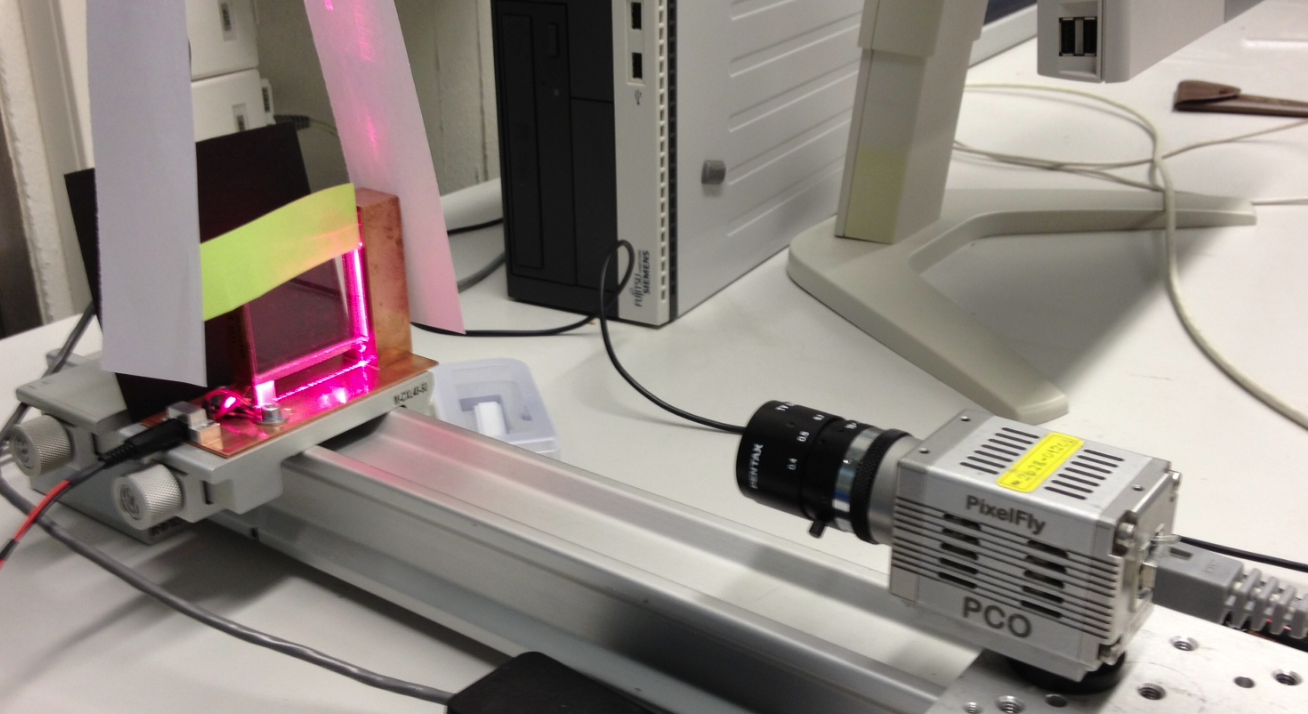
\includegraphics[width=\textwidth]{pics/setup1.png}
\caption{Experimental Set-up}
\label{pic:setup}
\end{figure}

The post processing is done with MATLAB. For the PIV part, we use a delivered MATLAB script. The script calculates the displacment of the tracers respectively the fluid particles. This allows us to display the velocity field, stream lines and some second order quantities like divergence and vorticity. Two sequences with different aperture settings are made and compared.

\section{Calculation of the frame separation time}

In order to have a significant displacement of the fluid particles or more precisely the tracers, we need to calculate the frame separation time. We assume that an average displacement of about $10\ pixels$ is needed for the PIV MATLAB script. As we know the average fluid velocity ($ v_{average} = 0.5\ mm/s$) and the wanted diplacement ($\Delta x_{pixel}=10\ pixel$), we can calculate the frame separation time from Equation \ref{eq:frseptime}.

\begin{equation}
v_{average}=\frac{\Delta x}{t_{separation}}=\frac{\kappa \Delta x_{pixel}}{t_{separation}}
\label{eq:frseptime}
\end{equation}

where $\kappa$ is the conversion factor ($[\frac{m}{pixel}]$) calcualted with $\kappa=\frac{l_{cell}}{width_{pixel}} = \frac{50 mm}{1280 pixel}=0.03907\ mm/pixel$.\\

The frame separation time is then $t_{separation}=0.7813\ s$ wich correponds to a frame rate of about $1.28\ frames/s$ . We use therefore frame 1 and 10 in the MATLAB PIV script for the calculation of the displacments.